% !TEX root = ./0.main.tex
在本节中,我们将阐述问题并详细介绍拟议的框架,并说明我们的框架与代表性的现有方法之间的区别。

\begin{table}
  \centering
  \caption{\label{tab:notation} 符号表.}
%   \small
%   \renewcommand{\arraystretch}{1.2}
  \begin{tabular}{c|p{2.55in}}
    \hline \hline
    \textbf{Notation} & \textbf{Description} \\
    \hline
    $u$ & 一个用户 \\
    $i$ & 一个项 \\
    $e$ & 一个交互 \\
    $\mathcal{U}$ & 用户集 \\
    $\mathcal{I}$ & 项集 \\
    % $\mathcal{E}$ & a user's sequence \\
    $\mathcal{I}_u$ & 用户的测试项集 $u$ \\
    % $\mathcal{D}$ & the set of training samples \\
    % $\mathcal{D}^{+/-}$ & the set of positive/negative training samples \\
    $d$ & 用户/项目嵌入的维度 \\
    $K$ & 兴趣嵌入的数量 \\
    $N$ & 候选项目数 \\
    $\mathbf{V}_u$ & 用户$u$ 的兴趣嵌入矩阵 \\
    $\delta(\cdot)$ & 指示函数 \\
    % $\mathbf{e}_i$ & the vector of primary capsule $i$ \\
    % $\mathbf{v}_j$ & the vector of interest capsule $j$ \\
    % $b_{ij}, c_{ij}$ & coupling coefficients of dynamic routing \\
    % $\mathbf{W}$ & transformation matrix \\
    \hline \hline
  \end{tabular}
\end{table}

\subsection{问题表述}
%~\cite{he2016fusing,hidasi2015session,rendle2010factorizing,smirnova2017contextual,tang2018personalized,tang2019towards}
% We formulate the \textit{sequential recommendation} problem as a sequence prediction problem. 
%recommend a set of items to each user that the user may be most interested in.
假设我们有一组用户 $u\in \mathcal{U}$ 和一组项目 $i\in \mathcal{I}$. 对于每个用户,我们都有一系列用户历史行为 $(e^{(u)}_{1}, e^{(u)}_{2}, \cdots, e^{(u)}_{n})$,按出现时间排序。$e^{(u)}_{t}$ 记录用户交互的第 $t^{th}$ 项。给定历史交互,\textit{顺序推荐}问题指预测用户可能会与之交互的下一个项目。
表~\ref{tab:notation} 中概述了用到的符号.

实际上,由于对延迟和性能的严格要求,工业推荐系统通常包括两个阶段,即匹配阶段和排名阶段。匹配阶段对应于检索前N个候选项目,而排名阶段用于按更精确的分数对候选项目进行排序。本文主要关注在匹配阶段提高有效性。在本节的以下部分中,我们将介绍可控制的多兴趣框架,并说明该框架对于\textit{顺序推荐}问题的重要性. % The overview of our models can be seen in Figure~\ref{fig:capsule}.

\begin{figure*}
    \centering
    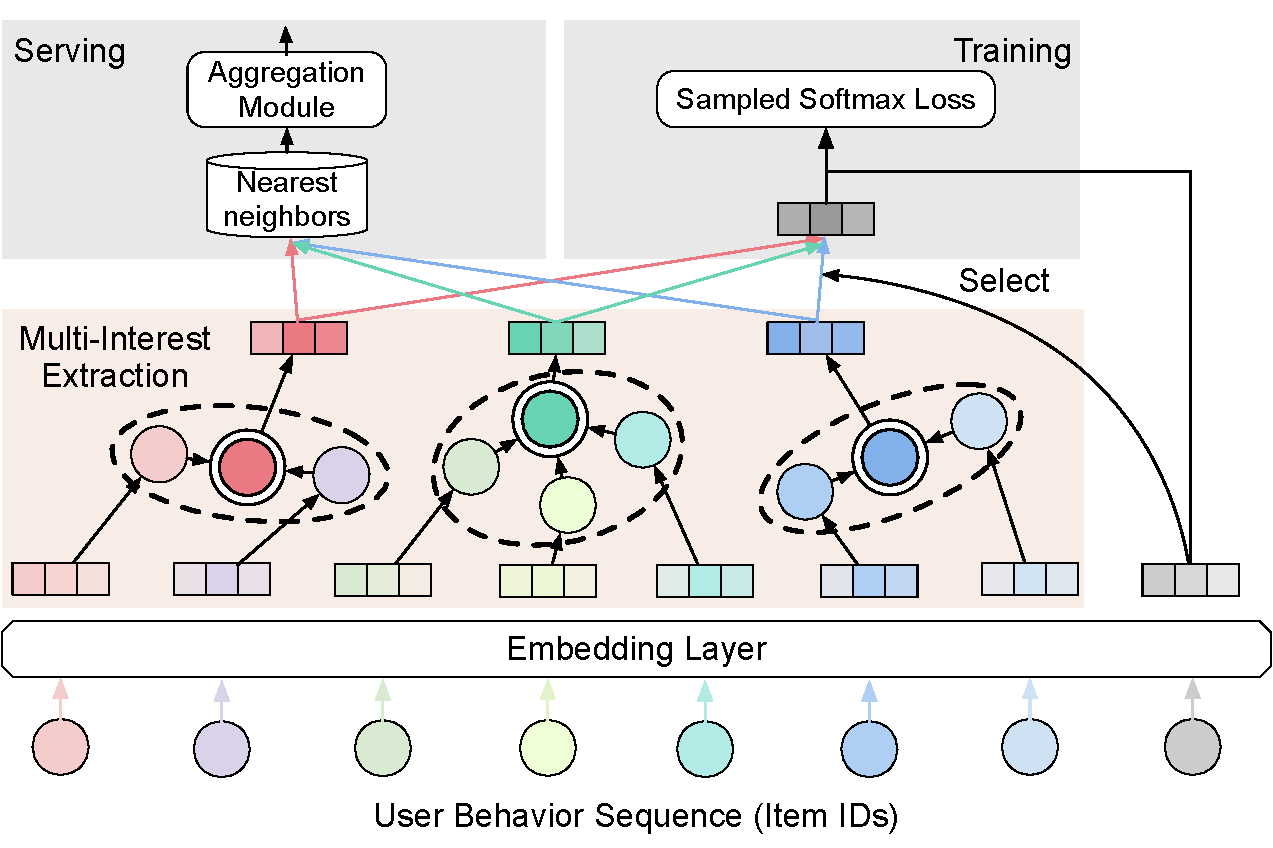
\includegraphics[width=0.8\textwidth]{figures/multi-interest-framework.pdf}
    \caption{顺序推荐模型的概述。我们模型的输入是用户行为序列,其中包含项ID的列表。该项目ID被送入嵌入层,并转化到该项目的嵌入。 兴趣嵌入是通过多兴趣提取模块生成的,然后可用于模型训练和服务。对于模型训练,将选择与目标嵌入最接近的兴趣嵌入来计算采样的softmax损失。为了提供服务,每个兴趣嵌入都将独立检索前N个最近的项目,然后将其馈入聚合模块。聚合模块通过可控制的过程来生成总体前N个项目,从而平衡推荐准确性和多样性。 }
    \label{fig:capsule_matching}
\end{figure*}

\subsection{多兴趣框架}
作为工业推荐系统的项目池通常由数百万甚至数十亿的项目,匹配阶段起着推荐系统至关重要的作用。 具体而言,匹配模型首先根据用户的历史行为来计算用户嵌入,然后基于用户嵌入为每个用户检索一组候选项目。借助快速K近邻算法(KNN)从大型项目池中选择最接近的项目以为每个用户生成候选集,我们主要集中在用户嵌入的计算上。换句话说,根据用户历史行为计算出的用户嵌入质量是匹配阶段的决定性因素。

现有的匹配模型通常使用RNN\cite{hidasi2015session,wu2017recurrent}为用户计算嵌入,但是大多数模型仅为每个用户生成一个嵌入向量。由于现实世界中的客户通常会考虑几种商品,而这些商品通常用于不同的用途,并且类别差异很大,因此,这种单一嵌入的方式缺乏足够的表达能力。 现实世界中客户的这种行为突显了需要使用多个向量来表示多重兴趣的重要性。基于这些考虑,我们为顺序推荐提出了一个多兴趣框架。我们框架的输入是用户行为序列,其中包含项目ID的列表,这些ID代表用户按时间顺序与商品的交互。商品ID被馈送到嵌入层,并转换为商品嵌入。多兴趣提取模块接收项目嵌入,并为每个用户生成多个兴趣。

%Interest capsules are generated through the dynamic routing method and can be then used for model training and online serving.

% RNN-based models~\cite{hidasi2015session,wu2017recurrent} are widely used in sequential recommendation. These models are effective for short-term user sequences~\cite{tang2019towards} but cannot capture long-term user interests from user sequences. 
要构建多兴趣提取模块,有很多可选的方法。 在本文中,我们探索了两种方法,即动态路由方法和自我关注方法,作为我们的多兴趣提取模块。 我们使用动态路由方法或自我关注方法的框架分别命名为 \model-DR 和 \model-SA.

\vpara{动态路由.}
%\zc{The motivation to exploit multi-interest network as the long-range model should be highlighted.}
我们将动态路由方法用作用户行为序列的多兴趣提取模块。 用户序列的项目嵌入可被视为主要胶囊,而多个用户兴趣可被视为兴趣胶囊。 我们使用CapsNet~\cite{sabour2017dynamic}中的动态路由方法. 
简要地说,我们使用动态路由来计算胶囊向量输入和输出。胶囊是一组神经元,其活动矢量代表特定类型的实体(例如对象或对象部件~\cite{sabour2017dynamic})的实例化参数。胶囊的输出矢量的长度表示由胶囊表示的实体在当前输入中的概率。令 $\mathbf{e}_i$ 为主要层的胶囊 $i$. 然后,我们基于主胶囊给出下一层胶囊 $j$ 的计算. 
%How to calculate capsules $\mathbf{v}_j$ of the output layer? 
我们首先将预测向量计算为
\begin{equation}
    \hat{\mathbf{e}}_{j|i}=\mathbf{W}_{ij} \mathbf{e}_{i},
\end{equation}
其中 $\mathbf{W}_{ij}$ 是转换矩阵。 那么,对胶囊 $j$ 的总输入就是所有预测矢量 $\hat{\mathbf{e}}_{j|i}$ 上的加权总和
\begin{equation}
        \mathbf{s}_j = \sum_i c_{ij} \hat{\mathbf{e}}_{j|i},
\end{equation}
其中 $c_{ij}$ 是由迭代动态路由过程确定的耦合系数。胶囊 $i$ 与下一层中所有胶囊之间的耦合系数总和为1. 我们使用初始 logits $b_{ij}$ 和“routing softmax”来计算耦合系数
\begin{equation}
    c_{ij}=\frac{\exp(b_{ij})}{\sum_k \exp(b_{ik})},
\end{equation}
其中 $b_{ij}$ 表示将胶囊 $i$ 和 $j$ 耦合的对数先验概率. 一个非线性“挤压”函数~\cite{sabour2017dynamic} 被提出来以确保短向量缩小到几乎为0的长度,长向量缩小到略小于1的长度. 胶囊 $j$ 的向量被计算为
\begin{equation}
    \label{eqn:squash}
    \mathbf{v}_j = \operatorname{squash}(\mathbf{s}_j) =  \frac{\|\mathbf{s}_j\|^2}{1+\|\mathbf{s}_j\|^2} \frac{\mathbf{s}_j}{\|\mathbf{s}_j\|},
\end{equation}
其中 $\mathbf{s}_j$ 是胶囊 $j$ 的总输入. 为了计算输出胶囊 $\mathbf{v}_j$, 我们需要根据 $\mathbf{v}_j$ 和 $\mathbf{e}_i$ 的内积来计算概率分布. $\mathbf{v}_j$ 的计算依赖与它自身;因此,动态路由方法被提出来解决这个问题. 整个动态路由过程在算法~\ref{algo:dynamic_routing}中给出. 然后用户 $u$ 的输出兴趣胶囊形成为下游任务的矩阵 $\mathbf{V}_u=[\mathbf{v}_1, ..., \mathbf{v}_K] \in \mathbb{R}^{d\times K}$.

% In order to ensure the diversity between interest capsules, we introduce a penalty term similar with \cite{lin2017structured}.

% \begin{equation}
%     P = \sum_{u\in \mathcal{U}}||\mathbf{V}_u \mathbf{V}_u^T-\mathbf{I}||_F^2
% \end{equation}
% where $||\cdot||_F$ denotes the Frobenius norm of a matrix. The penalty term $P$ will be multiplied by a coefficient and then added to the original loss (binary cross entropy loss or sampled softmax loss).

\begin{algorithm}[t]
	\caption{动态路由 \label{algo:dynamic_routing}}
	\KwIn{primary capsules $\mathbf{e}_i$, iteration times $r$, number of interest capsules $K$}
	\KwOut{interest capsules $\{\mathbf{v}_j, j=1,...,K\}$}
	for each primary capsule $i$ and interest capsule $j$: initialize $b_{ij} = 0$. \\
    \For{$iter = 1,\cdots,r$} {
        for each primary capsule $i$: $\mathbf{c}_i = \operatorname{softmax}(\mathbf{b}_{i})$.\\
        for each interest capsule $j$: $\mathbf{s}_j = \sum_{i} c_{ij}\mathbf{W}_{ij}\mathbf{e}_i$.\\%\hat{\mathbf{e}_{j|i}}$. \\

        for each interest capsule $j$: $\mathbf{v}_j = \operatorname{squash}(\mathbf{s}_j)$. \\

        for each primary capsule $i$ and interest capsule $j$: $b_{ij} = b_{ij}+ \mathbf{v}_j^\top \mathbf{W}_{ij}\mathbf{e}_i$.
    }
    \Return{$\{\mathbf{v}_j, j=1,...,K\}$}
\end{algorithm}


\vpara{自注意力方法.} 
自注意力方法~\cite{lin2017structured} 同样也可以被运用与我们的多兴趣提取模块。
给出用户的行为嵌入, $\mathbf{H}\in \mathbb{R}^{d\times n}$, 其中 $n$ 是用户序列的长度, 我们使用自注意力机制来获得一个权重向量 $\mathbf{a} \in \mathbb{R}^{n}$:
\begin{equation}
    \mathbf{a} = \operatorname{softmax}(\mathbf{w}_{2}^\top \operatorname{tanh}(\mathbf{W}_{1} \mathbf{H}))^\top,
\end{equation}
\noindent 其中 $\mathbf{w}_{2}$ 和 $\mathbf{W}_{1}$ 是可训练的参数,大小分别是为 $d_a$ 和 $d_a \times d$。 上标 $\top$ 表示向量或矩阵的转置。大小为 $n$ 的向量 $\mathbf{a}$ 表示用户行为的注意权重。 当根据注意力权重来总结用户行为的嵌入时,我们可以为用户获得向量表示 $\mathbf{v}_u = \mathbf{H} \mathbf{a}$ 。 对于利用用户序列顺序的自注意方法,我们将可训练的位置嵌入~\cite{vaswani2017attention} 添加到输入嵌入中。 位置嵌入与项目嵌入具有相同的尺寸 $d$ ,并且可以直接将两者相加。

该矢量表示关注并反映用户 $u$ 的特定兴趣。为了代表用户的整体兴趣,我们需要从关注不同兴趣的用户行为中获取多个 $\mathbf{v}_u$ 。因此,我们需要进行多次注意力。 我们将 $\mathbf{w}_{2}$ 扩展为 $\mathbf{W}_{2}$ 到 $d_a$-by-$K$ 的矩阵中。然后注意向量 $\mathbf{a}$ 变为注意矩阵 $\mathbf{A}$ 作为
\begin{equation}
    \mathbf{A} = \operatorname{softmax}(\mathbf{W}_{2}^\top \operatorname{tanh}(\mathbf{W}_{1} \mathbf{H}))^\top.
\end{equation}

用户兴趣最终矩阵 $\mathbf{V}_u$ 可以被这样计算
\begin{equation}
    \label{eqn:sa}
    \mathbf{V}_u = \mathbf{H} \mathbf{A}.
\end{equation}



\vpara{模型训练.}
在通过多兴趣提取模块根据用户行为计算出兴趣嵌入后,我们使用 \textit{argmax} 运算符为目标商品 $i$ 选择相应的用户嵌入向量:

\begin{equation}
    \label{eqn:argmax}
    \begin{aligned}
        % \mathbf{v}_u & = \operatorname{Attention}(\mathbf{e}_i, \mathbf{V}_u, \mathbf{V}_u) \\
        % & = \mathbf{V}_u \operatorname{softmax}(\mathbf{V}_u^\top \mathbf{e}_i),
        \mathbf{v}_u = \mathbf{V}_u[:, \operatorname{argmax}(\mathbf{V}_u^\top \mathbf{e}_i)],
    \end{aligned}
\end{equation}
其中 $\mathbf{e}_i$ 表示目标项目 $i$ 的嵌入,而 $\mathbf{V}_u$ 是由用户兴趣嵌入形成的矩阵 %The function $\operatorname{pow}$ is the element-wise exponential function and $p$ is a hyperparameter which controls the attention distribution. 

给定训练样本 $(u,i)$ ,用户嵌入 $\mathbf{v}_u$ ,项目嵌入 $\mathbf{e}_i$ ,我们可以计算用户 $u$ 与物品 $i$ 交互的可能性:

\begin{equation}
    \label{eqn:likelihood}
    P_\theta(i|u) = \frac{\exp(\mathbf{v}_u^\top \mathbf{e}_i)}{\sum_{k\in\mathcal{I}}\exp(\mathbf{v}_u^\top \mathbf{e}_k)}.
\end{equation}

我们模型的目标函数是最小化如下的负对数相似性

\begin{equation}
    \label{eqn:loss}
    loss = \sum_{u\in \mathcal{U}} \sum_{i\in \mathcal{I}_u} -\log P_\theta(i|u).
\end{equation}

方程 (\ref{eqn:likelihood}) 的和运算消耗很大;因此,我们用了一个简单的softmax方法 ~\cite{jean2014using, covington2016deep} 来训练我们的模型

\vpara{在线服务.}
对于在线服务,我们使用多兴趣提取模块为每个用户计算多个兴趣。 用户的每个兴趣向量都可以通过最近的邻居库(例如Faiss〜\ cite {JDH17})从大型项目池中独立检索前N个项目。 由多个兴趣检索的项目将被馈送到聚合模块中,以确定整体候选项目。 最后,将为用户推荐评分较高的项目。


% \subsection{Multi-Interest Extraction Module}


\begin{algorithm}[t]
	\caption{Greedy Inference \label{algo:greedy_infer}}
	\KwIn{Candidate item set $\mathcal{M}$, number of output items $N$}
	\KwOut{Output item set $\mathcal{S}$}
	$\mathcal{S} = \varnothing$ \\
    \For{$iter = 1,\cdots,N$} {
        $j = \operatorname{argmax}_{i \in \mathcal{M} \backslash \mathcal{S}} \left( f(u, i) + \lambda \sum_{k \in \mathcal{S}} g(i,k) \right)$ \\
        $\mathcal{S} = \mathcal{S} \cup \{j\}$
    }
    \Return{$\mathcal{S}$}
\end{algorithm}

\subsection{聚合模块}
在多兴趣提取模块之后,我们根据每个用户的过去行为为其获取多个兴趣嵌入。 每个兴趣嵌入都可以根据内部生产邻近性独立检索前N个项目。 但是,如何汇总这些来自不同兴趣的项目以获取总体前N个项目? 一种基本且直接的方法是根据商品的内部生产接近度和用户兴趣来合并和过滤商品,可以将其形式化为
\begin{equation}
    f(u,i) = \max_{1\leq k\leq K}(\mathbf{e}_i^\top \mathbf{v}_u^{(k)}),
\end{equation}
其中 $\mathbf{v}_u^{(k)}$ 是用户 $u$ 的第k个兴趣嵌入。 这是用于聚合过程以最大化推荐准确性的有效方法。 但是,这不仅仅涉及当前推荐系统的准确性。 人们更有可能被推荐新颖或多样化的东西。
问题可以被下面这样公式化。给定一个集合 $\mathcal{M}$ 带有 $K\cdot N$ 物品,获取自用户 $u$ 的 $K$ 个兴趣,找到一个集合 $\mathcal{S}$ 带有 $N$ 个项目使得预定义的值函数最大化。我们的框架使用可控制的过程来解决此问题。 我们使用以下值函数 $Q(u,S)$ 通过可控制因子 $\lambda \geq 0$ 平衡推荐的准确性和多样性,
\begin{equation}
    Q(u,\mathcal{S}) = \sum_{i\in \mathcal{S}} f(u,i) + \lambda \sum_{i\in \mathcal{S}} \sum_{j\in \mathcal{S}} g(i,j).
\end{equation}
\noindent 这里 $g(i,j)$ 是多样性或不相似函数,例如
\begin{equation}
    g(i,j) = \delta(\operatorname{CATE}(i) \neq \operatorname{CATE}(j)).
\end{equation}
其中 $\operatorname{CATE}(i)$ 表示项目 $i$ 的类别, $\delta(\cdot)$ 是一个指示函数。
对于最准确的情况,即 $\lambda=0$ ,我们仅使用上述简单方法即可获得整体商品。 对于最多样化的情况,即, $\lambda=\infty$ ,可控模块为用户找到最多样化的商品。 我们在~\ref{sec:control_study}中研究可控因素。 我们提出一种贪婪推断算法,以近似最大化值函数 $Q(u,S)$,该算法被列在~\ref{algo:greedy_infer}中。


\subsection{与现有模型的连接}
我们对我们的模型和现有模型做了一个比较

\vpara{MIMN.}
MIMN~\cite{pi2019practice},推荐排名的最新代表作品是使用内存网络从长序列行为数据中捕获用户兴趣。 MIMN和我们的模型都针对用户的多重兴趣。 对于非常长的顺序行为,基于内存的体系结构可能也不足以捕获用户的长期利益。 与MIMN相比,我们的模型利用多兴趣提取模块来利用用户的多兴趣,而不是使用具有内存利用率正则化和内存归纳单元的复杂内存网络。

\vpara{MIND.}
MIND~\cite{li2019multi},是推荐匹配阶段的一项最新代表作品,提出了一种“兴趣转化为行为” (B2I) 动态路由,用于将用户的行为自适应地汇总到兴趣表示向量中。 与MIND相比, \model-DR 遵循 CapsNet~\cite{sabour2017dynamic}使用的原始动态路由方法,该方法可以捕获用户行为的顺序信息。 我们的框架还探索了一种多关注点提取的自我关注方法。 此外,我们的框架利用可控的汇总模块来根据用户的多重兴趣来平衡推荐的准确性和多样性。

% Specifically, MIND uses fully shared transformation matrices, i.e., $\mathbf{W}_{ij}=\mathbf{W}$. In this situation, B2I dynamic routing ignores the item positions and considers the item sequence as an item set. However, the item positions are important for the sequential recommendation. 
%In this situation, the logits $b_{ij}$ cannot be initialized as zeros and are randomly initialized as Gaussian distribution for each batch, which may impact the semantics of capsules. 
% Our method uses partially shared transformation matrices, i.e., $\mathbf{W}_{ij}=\mathbf{W}_j$. 
%% vim: formatoptions=
